%!TEX root = ../documentation.tex

%% SECTION
\section{Zusammenarbeit in ausgewählten Vorgehensmodellen}
\label{sec:zusammenarbeit}


Im Folgenden werden die vier Vorgehensmodelle \emph{Wasserfallmodell}, \emph{V-Modell}, \emph{Rational Unified Process} und \emph{Scrum} in Bezug auf die Zusammenarbeit kurz vorgestellt und miteinander verglichen.


%% SUBSECTION
\subsection{Wasserfall-Modell}
\label{sec:zusammenarbeit:wasserfall}
Das Wasserfallmodell wurde im Jahr 1970 von Dr. Winston W.Royce in einem Paper vorgestellt. Somit ist dieses Modell auch einer der ältesten und bekannten Vorgehensmodellen in der Softwareentwicklung. 
Trotz des Alters findet das Modell immer noch Einsatz in vielen großen Unternehmen \cite{IJC:2015:Related:}\cite{TryQA:24102022:What:1}.
\\Das Vorgehensmodell stellt die Projektphasen in einem \glqq Wasserfall\grqq{} dar. Dabei werden die einzelnen Phasen top-down nacheinander abgearbeitet und sind in sich abgeschlossen. 
Das heißt, dass bevor eine Phase komplett abgearbeitet wird, darf die Nächste nicht angefangen werden. Darüber hinaus lässt das reine Wasserfall-Modell keine Rückführung zu den vorherigen, abgeschlossenen Phasen, zu \cite[84]{Goll:2011:Methoden:}. 
\\
Als Grundlage für den gesamten Entwicklungsprozess dient die Spezifikation. So werden auch die Anforderungen für Anwender von vornherein ermittelt und festgeschrieben. 
Die Ergebnisse einer Phase fallen in die nächste, um dort weiterverarbeitet zu werden. Zur Kommunikation zwischen den Entwicklern und Anwendern werden umfangreiche Dokumente über das Softwaresystem erstellt \cite[83]{Goll:2011:Methoden:}. 
Die wichtigsten Phasen des Modells lassen sich folgendermaßen definieren\cite[85]{IJC:2015:Related:}\cite{Goll:2011:Methoden:}: 
\begin{enumerate}
    \item Anforderungsdefinition: in Zusammenarbeit mit dem Kunden werden die Spezifikationen, Ziele und Anforderungen an den Softwareprodukt definiert. Anschließend wird eine umfassende Dokumentation erstellt, die die Grundlage der weiteren Arbeit bildet. 
    \item Software- und System-Entwurf: die Anforderungen werden bearbeitet und es werden abstrakte Softwarekomponenten sowie die grundlegende Softwarearchitektur modelliert
    \item Implementierung: in dieser Phase werden die modellierten Software-Komponenten programmiert. 
    \item Integration und Testen: die einzelnen Elemente des Software-Systems werden zusammengeführt und es werden Tests durchgeführt.
    \item Betrieb und Wartung: das erstellte Produkt wird zum Gebrauch freigegeben.
\end{enumerate}
Das Wasserfallmodell, bereits in der einfachen Ausführung, bietet eine gute Möglichkeit, die Anwenderteams bei kleineren Projekten wie z.B. Prototypen, zu organisieren. 
Darüber hinaus lässt sich das Modell durch weitere Funktionalitäten erweitern. Zum Beispiel, um die Qualität der Software zu verbessern und eine höhere Flexibilität in die Projekte zu schaffen, wurde das sogenannte \glqq Wasserfallmodell mit Rückführschleifen\grqq{} entwickelt.
Dabei finden Validierungen und Verifikationen der vorherigen Phase beim Übergang in die nächste Phase statt und es lässt sich ein \glqq Rückschritt\grqq{} über mehrere Phasen implementieren \cite[86,87]{Goll:2011:Methoden:}.
Die graphische Abbildung des oben beschriebenen Modells wird in Abbildung \ref{fig:waterfallModel} dargestellt. Dabei wird das einfache Wasserfallmodel mit den roten Pfeilen und das erweiterte mit blauen dargestellt.   
\begin{figure}
\centering
    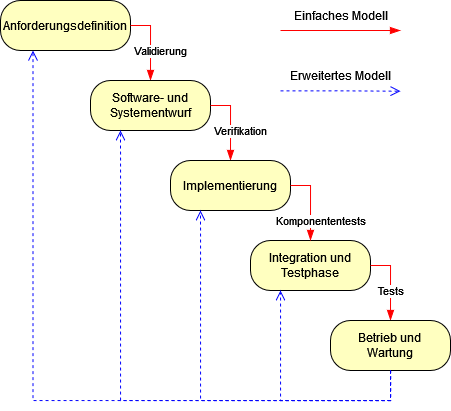
\includegraphics[width=0.7\textwidth, height=0.7\textheight,keepaspectratio]{WaterfallModel.png} 
    \caption{Das einfache Wasserfallmodell}
    \label{fig:waterfallModel}
\end{figure}
\\
Die Vorteile des Wasserfallmodells liegen in der klaren, einfachen Struktur des Modells. Die Abläufe werden klar und verständlich in Phasen aufgeteilt wodurch sich die Ergebnisse kontrollieren lassen.
Dadurch können die Aufgaben während einer Phase klar auf die Entwicklerteams aufgeteilt und verwaltet werden und jede Phase kann fehlerarm ablaufen. Darüber hinaus lässt sich das Modell mithilfe verschiedener Ansätze
erweitern wodurch verschiedene Aspekte der Verwaltung und Softwareentwicklung, z.B. Qualitätssicherung verbessert werden \cite[84-87]{Goll:2011:Methoden:} \cite[14]{Kyer:2019:Overview:}.  
\\Die Nachteile des Modells basieren zum einen auf der Starrheit und zum anderen auf dem viel zu großem Anteil der Dokumentation in dem Modell.
Aufgrund der Starrheit lässt sich nicht so schnell auf die Veränderungen der Anforderungen und Spezifikation reagieren und dadurch können erhebliche Zeit- und Geldkosten anfallen. 
Dieses Problem wird zwar teilweise durch das erweiterte Wasserfall Modell gelöst, jedoch genügt es nicht ganz, wenn die Anforderungen oft verändert werden müssen. Die Dokumentation, die umfänglich während des Projektablaufs geführt wird, 
kann auch unter Umständen einen viel zu großen Stellenwert im Projekt übernehmen, wodurch die eigentlichen Ziele nicht vollständig erreicht werden \cite[14]{Kyer:2019:Overview:} \cite{IJC:2015:Related:}.
\\Bezogen auf die Zusammenarbeit, verfügt das Modell über zwei Ansätze: es findet ein Austausch zwischen Entwicklern innerhalb eines Teams während einer Phase und eine Kommunikation mithilfe von Dokumenten zwischen verschiedenen Phasen. 
Durch diese Ansätze kann zwar eine verständliche, fest vorgegebene Kommunikation geführt und eine Kontrolle angesetzt werden, aber bei größeren Projekten, kann dies zu einer langen Projektlaufzeit führen. 
Die Starrheit des Modells wird dabei nicht aufgelöst, was zu großen Problemen bei Anforderungsänderungen und anderen ungeplanten Geschehen führen kann. 

\subsection{V-Modell}
\label{sec:zusammenarbeit:vModell}
Ein weiteres sequenzielles Modell, welches heutzutage häufig in deutschen Behörden und großen Unternehmen verwendet wird, ist das V-Modell \cite{Hohn:2008:V:}. 
Wie der Name bereits bezeichnet, werden die einzelnen Projektphasen im Modell in Form eines \glqq V\grqq{} dargestellt. 
Das V-Modell wurde als Weiterentwicklung des Wasserfallmodels entwickelt und liegt dabei den Fokus vor allem auf der Qualitätssicherung. 
Diese wird durch Einführung der Verifikation und Validierung mithilfe von Tests nach jeder Projektphase ermöglicht \cite{TryQa:24102022:What:2}\cite{Vans:2014:Software:}.
\\Das V-Modell entstand bereits in 80er Jahren und stellte als Modell-Prototyp den Grundgerüst der modernen Vorgehensmodelle für die Bundeswehr in Deutschland her \cite[1]{Dros:1999:V:}.
Dieser Prototyp wurde im Laufe der Jahre bearbeitet und im Jahr 1992 für alle Bundesbehörden in Deutschland in einer verbindlichen Fassung als Rahmenregelung empfohlen \cite[3]{Dros:1999:V:}. 
Diese Fassung beschrieb den Arbeitsprozess „statisch, als Abfolge einzelner Arbeitsschritte“ \cite{Dros:1999:V:}(S 3) wodurch dynamische Aspekte des Entwicklungsprozesses 
wie z.B. Kombinierung der verschiedenen Phasen miteinander, unbeschrieben wurden. Dieses und andere Probleme des Modells führten dazu, dass das Modell überarbeitet und weiterentwickelt werden musste. 
Dies führte zur Standardisierung des V-Modells 97 im Jahre 1997 \cite[3,4]{Dros:1999:V:}.  
Die neuen Projekte und Entwicklungen in Methodik und Technologie wurden in diesem Modell dennoch unzureichend beschrieben und konnten somit nicht dem Stand der Technik entsprechen. 
Als Antwort auf diese Probleme wurde im Jahre 2004 das V-Modell XT vorgestellt. XT steht dabei für \glqq extreme Tailoring\grqq{} (\glqq extremes Maßschneidern\grqq{}) und drückt die angestrebte Flexibilität 
des Modells aus \cite[3]{Hohn:2008:V:}. Das V-Modell XT ist die neueste Version des V-Modells und wird fortlaufend aktualisiert. Diese Version wird im Folgenden näher beschrieben. 
\\

Das V-Modell XT beschreibt die Erstellung eines IT-Systems als eine Folge von Aktivitäten, bei denen Produkte erstellt werden \cite[4]{Dros:1999:V:}. 
Nach dem Erstellen eines Produktes wird dieser gegen die gestellten Anforderungen geprüft (\textbf{Verifikation})\cite[107]{Frie:2009:V:}. 
Zum anderen, ist auch zu prüfen, ob das erstellte Produkt für die vorgesehene Aufgabe geeignet ist, also ob z.B. das richtige System in Auftrag gegeben wurde. (\textbf{Validierung})
In der Software-Entwicklung erfolgt die \textbf{Verifikation} durch die ausgebildeten Prüfer, welche bei der Übergabe der Produkte, 
die in Form von formalen Dokumenten bestehen, mitwirken \cite[36,37]{Hohn:2008:V:} \cite[107]{Frie:2009:V:}. 
Die \textbf{Validierung} erfolgt dabei oft mithilfe des „Test-first“ Ansatzes. Dabei werden, angefangen bereits bei der Anforderungsdefinition bis hin zur Implementierungsphase, Tests und Abnahmekriterien 
für die Projektbausteine definiert \cite[2]{Vans:2014:Software:}. 
\\Insgesamt lässt sich das Modell wie in Abbildung \ref{fig:v_model_xt} beschreiben. Dabei findet in dem Modell von Oben nach Unten eine schrittweise Verfeinerung des Gesamtsystems. 
Am Anfang findet eine Anforderungsdefinition, die dann bis zum Modulentwurf und deren Implementierung zerlegt wird. Nachdem man dann im Modell unten \glqq angekommen ist\grqq{}, 
wird das System wieder rekursiv aufgebaut und dabei die vorher geschriebenen Tests bis zur Abnahme durchgeführt \cite[93]{Goll:2011:Methoden:}\cite{Lude:2007:Software:}.  
\begin{figure}
\centering
    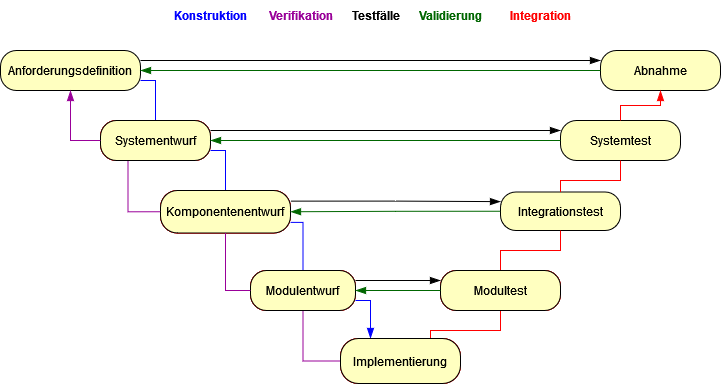
\includegraphics[width=\textwidth, height=\textheight,keepaspectratio]{V_Model_XT.png} 
    \caption{Vereinfachte Darstellung des V-Modells XT}
    \label{fig:v_model_xt}
\end{figure}
Das V-Modell XT ist insgesamt in 4 Submodelle gegliedert. Das im Bild \ref{fig:v_model_xt} dargestelltes Modell beschreibt dabei das Submodell „Softwareentwicklung“. 
Zu den weiteren Tätigkeiten gehören: Qualitätssicherung, Konfigurationsmanagement und das Projektmanagement. Die Vier Modelle sind miteinander verbunden, und sorgen zusammen für einen kontrollierten, 
sicheren Projektablauf \cite[6]{Frie:2009:V:} \cite[4]{Dros:1999:V:}. 
\\
Der Kernunterschied des V-Modells XT zu ihrem Vorgänger, dem V-Modell XT liegt in der Anpassbarkeit und Flexibilität. Dabei wurde das Modell so entwickelt, dass es für verschiedenen Projekten 
angewendet werden kann. Zu den Maßnahmen gehören zum Beispiel, die anpassbare Größe der Dokumentation, damit „so viel … wie nötig, aber so wenig wie möglich“ erzeugt wird \cite[3]{Frie:2009:V:}. 
Darüber hinaus lässt sich in dem Modell die Anzahl von Phasen oder Vorgehensbausteinen und die Zuordnung von Mitarbeiter-Rollen jeweils spezifisch für das Projekt zuordnen. Diese Methode wird als „Tailoring“ 
bezeichnet. \cite[6]{Frie:2009:V:}
\\
Insgesamt lässt sich sagen, dass das Modell gut für verschiedene Projekttypen und -Größen einsetzbar ist \cite[3]{Frie:2009:V:}. 
Wie bereits oben beschrieben, findet das V-Modell insbesondere in der Industrie und bei IT-Projekten der Bundesbehörden Einsatz. 
Darüber hinaus, lassen sich verschiedene Projektdurchführungsstrategien innerhalb des V-Modells auswählen, z.B. iterativ oder evolutionär, welche für unterschiedliche Arten von Projekten anwendbar sind \cite[7]{Hohn:2008:V:}. 
Insbesondere kann das Modell in Projekten verwendet werden, die feste, verständliche und wenig veränderbare Anforderungen haben \cite{Vans:2014:Software:}. Die Größe dieser Projekte sollte auch nicht zu gering sein, weil ein großer Aufwand in der Planung eingesetzt werden muss.
\\
Die Vorteile des Modells liegen in der Qualitätssicherung und strikten Kontrolle innerhalb des Modells. 
Die häufige Verwendung des „Test First“ Ansatzes und die Maßnahmen zur Verifikation und Validierung ermöglichen einen fehlerarmen Ablauf des Projekts und die Erstellung eines qualitativ hohen Endprodukts. 
Durch das neu eingeführte „Tailoring“ im V-Modell XT ist das Modell auch flexibler geworden und kann somit für verschiedene Projekte benutzt werden. 
\\Die Nachteile des Modells leiten sich vor allem aus der Starrheit des Modells heraus. Da das Modell linear ist, können die einzelnen Projektphasen nach dem das Projekt angefangen ist, nicht einfach umstrukturiert werden. 
Darüber hinaus müssen bei dem Modell die Anforderungen strikt formuliert werden, da die Änderungen dieser schwer in der Mitte des Projekts umgesetzt werden. \cite{TryQa:24102022:What:2} \cite{Buns:2008:Vorgehensmodelle:}
\\Wie bereits oben beschrieben, ist das V-Modell in 4 Submodelle gegliedert. Dadurch lassen sich die Rollen der Qualitätsmanager, der Softwarearchitekten und anderen Mitarbeiter voneinander trennen und 
jeder Mitarbeiter befindet sich in seinem Zuständigkeitsgebiet. Die Kommunikation wird dabei wie bei dem Wasserfallmodell mithilfe von Dokumenten geregelt. Darüber hinaus lassen sich unterschiedliche Arten von Austausch
in Unternehmen regeln. 